%!TEX root = ../main.tex

\section{开胃菜}
\subsection{简单的分类问题}
\begin{frame}{\insertsection}{\insertsubsection}
\begin{minipage}[m]{0.48\textwidth}
在二维空间中, 有 $500$ 个点, 这 $500$ 个点被分成两类, 一类被标记为绿色, 一类被标记为蓝色, 如右图所示.

现在的问题是, 计算机如何根据已有的数据, 找到一个分类的方法, 可以在给定 $(x_1, x_2)$ 时, 会判断点 $(x_1, x_2)$ 的颜色.

计算机解决二分类的方法有很多, 在这里, 介绍一种基于神经网络的方法, 来解决这个问题, 来帮助大家理解机器学习的过程.
\end{minipage}%
\hfill%
\begin{minipage}[m]{0.48\textwidth}
\begin{tikzpicture}
  \begin{axis}[%
    xlabel = $x_1$,
    ylabel = $x_2$,
    height = 7.8cm,
    width = 7cm,
    title = $500$ 个点的分布图
  ]
    \addplot[only marks, discard if not={type}{1}, blue] table[col sep=comma, x = x1, y = x2]{../../src/classification/training.dat};
    \addplot[only marks, discard if not={type}{0}, green] table[col sep=comma, x = x1, y = x2]{../../src/classification/training.dat};
  \end{axis}
\end{tikzpicture}
\end{minipage}
\end{frame}

\subsection{建立神经网络}
\begin{frame}{\insertsection}{\insertsubsection}
我们不妨设绿色为 $1$, 蓝色为 $0$, 那么, 问题就变成了找到一个坐标 $(x_1, x_2)$ 到颜色 $y$ 的一个映射关系 $y = h(x_1, x_2)$.\vspace{10pt}

\begin{minipage}[m]{0.55\textwidth}
为此, 我们建立一个简单的神经网络, 如图所示.
\begin{center}
\scalebox{0.8}{%
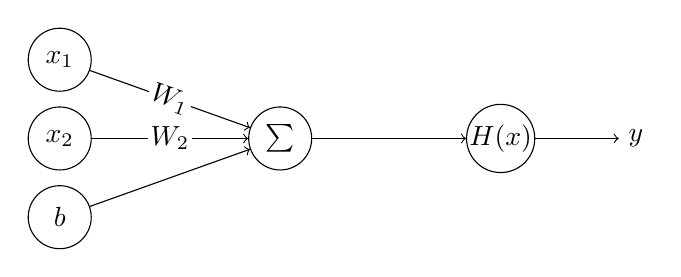
\begin{tikzpicture}[%
  node/.style = {circle, draw, inner sep = 0pt, minimum size = 0.8cm},
  x = 1.4cm]
  \node[node] (x1) at (0, 2) {$x_1$};
  \node[node] (x2) at (0, 1) {$x_2$};
  \node[node] (b)  at (0, 0) {$b$};
  \node[node] (sum) at (2, 1) {$\sum$};
  \node[node] (step) at (4, 1) {$H(x)$};

  \draw[->] (x1) -- (sum) node[midway, fill = white, inner sep = 1pt, sloped] {$W_1$};
  \draw[->] (x2) -- (sum) node[midway, fill = white, inner sep = 1pt, sloped] {$W_2$};
  \draw[->] (b) -- (sum);
  \draw[->] (sum) -- (step);
  \draw[->] (step) -- ++(0:1.5cm) node[anchor = west] {$y$};
\end{tikzpicture}}
\end{center}
因此, 我们可以得到神经网络的表达式:\vspace{-10pt}
\begin{align*}
  y &= H(W_1x_1 + W_2x_2 + b) = H(W_1x_1 + W_2x_2 + 1)\text{,}\\
    &= H(\bm{W}\bm{x} + 1)\text{.}
\end{align*}
\end{minipage}%
\hfill%
\begin{minipage}[m]{0.43\textwidth}
\begin{tikzpicture}
  \begin{axis}[width = \textwidth,
               height = 5.7cm,
               xlabel = $x$,
               ylabel = $H(x)$,
               title = 单位阶跃函数图像]
    \addplot[mark = none, samples = 100, blue] {x > 0};
  \end{axis}
\end{tikzpicture}
\end{minipage}
\end{frame}

\subsection{确定目标函数}
\begin{frame}{\insertsection}{\insertsubsection}
所谓目标函数, 就是当目标函数取得最值的时候, 神经网络最符合我们的预期. 换句话就是, 目标函数就是衡量神经网络好坏指标.

我们这里采用所有样本都分类成功的概率作为目标函数:
\[
p(X) = \prod_{i = 1}^{500} p(X_i)\text{,}
\]

对于第 $i$ 个坐标 $\bm{x}_i = (x_{i, 1}, x_{i, 2})$,其正确值是 $y_i$,那么当曲线 $h(x_1, x_2)$ 给定的情况下,其作出正确分类的概率为%
%
\begin{align*}
  p(X_i) &= \left\{
  \begin{array}{ll}
    1, & \text{$H(\bm{W}\bm{x}_i + 1) = 1, y = 1$ 或者 $H(\bm{W}\bm{x}_i + 1) = 0, y = 0$,}\\
    0, & \text{$H(\bm{W}\bm{x}_i + 1) = 0, y = 1$ 或者 $H(\bm{W}\bm{x}_i + 1) = 1, y = 0$.}
  \end{array}
  \right.
\end{align*}
\end{frame}

\begin{frame}{\insertsection}{\insertsubsection}
接下来, 需要对这个式子进行化简.
\[
  p(X_i) = \left\{
  \begin{array}{ll}
    1, & \text{$H(\bm{W}\bm{x}_i + 1) = 1, y = 1$ 或者 $H(\bm{W}\bm{x}_i + 1) = 0, y = 0$,}\\
    0, & \text{$H(\bm{W}\bm{x}_i + 1) = 0, y = 1$ 或者 $H(\bm{W}\bm{x}_i + 1) = 1, y = 0$.}
  \end{array}
  \right.
\]

我们可以注意到, 当 $y = 1$ 时, $p(X_i)$ 的值与 $H(\bm{W}\bm{x}_i + 1)$ 一致; 当 $y = 0$ 时, $p(X_i)$ 的值与 $H(\bm{W}\bm{x}_i + 1)$ 和为 $1$, 于是有:
\[
  p(X_i) = \left\{
  \begin{array}{ll}
    H(\bm{W}\bm{x}_i + 1), & y = 1\text{,}\\
    1 - H(\bm{W}\bm{x}_i + 1), & y = 0\text{.}
  \end{array}
  \right.
\]

注意到 $\forall x \in \mathbb{R}$ 都有 $x^0 = 1$,还可以将上式继续化简为:
\[
  p(X_i) = H(\bm{W}\bm{x}_i + 1)^{y_i}\cdot\big(1 - H(\bm{W}\bm{x}_i + 1)\big)^{1 - y_i}\text{.}
\]
\end{frame}

\begin{frame}{\insertsection}{\insertsubsection}
因此, 我们的目标函数就确定下来了:
\[
  p(X) = \prod_{i = 1}^{500} H(\bm{W}\bm{x}_i + 1)^{y_i}\cdot\big(1 - H(\bm{W}\bm{x}_i + 1)\big)^{1 - y_i}\text{.}
\]

为了方便计算, 对上式左右两边都取以 $\e$ 为底的对数:
\[
  \ln p(X) = \sum_{i = 1}^{500} y_i\ln H(\bm{W}\bm{x}_i + 1) + (1 - y_i)\ln\big(1 - H(\bm{W}\bm{x}_i + 1)\big)\text{.}
\]

但是, 上述目标函数还存在问题:%
%
\begin{itemize}
\item 导致函数 $\ln p(X)$ 不可微, 不能采用梯度下降法来计算函数的最值(其实是极值);
\item 只要有一个预测错误, 函数 $\ln p(X) = -\infty$, 目标函数并不能衡量模型的精度.
\end{itemize}
\end{frame}

\begin{frame}{\insertsection}{\insertsubsection}
解决方法就是用 Sigmoid 函数 $g(\,\cdot\,)$ 代替上式中的单位阶跃函数 $H(\,\cdot\,)$, 原因有:
\begin{itemize}
\item Sigmoid 函数与单位阶跃函数形状非常相似, 并且值域为 $(0, 1)$, 不会导致目标函数出现 $-\infty$ 的情况, 其函数图像如右图所示.
\end{itemize}\vspace{-10pt}
\begin{minipage}[t]{0.48\textwidth}
\begin{itemize}
\item Sigmoid 处处可微, Sigmoid 的表达式为:%
\[
  g(x) = \frac{1}{1 + \exp(-x)}\text{.}
\]
\item Sigmoid 函数有非常好的导函数性质, 有:%
\[
  \frac{\dif g(x)}{\dif x} = g(x)\cdot\big(1 - g(x)\big)\text{.}
\]
\end{itemize}
\end{minipage}%
\hfill%
\begin{minipage}[t]{0.48\textwidth}
\begin{figure}
  \centering\vspace{-20pt}
  \begin{tikzpicture}
    \begin{axis}[height = 4.5cm,
                 width = \textwidth,
                 xlabel = $x$,
                 title = Sigmoid 函数与单位阶跃函数图像,
                 legend pos = north west,]
      \addplot[mark = none, blue, domain = -30:30, samples = 100] {(x > 0)};
      \addplot[mark = none, green, domain = -30:30, samples = 100] {(x <= 0) * exp(x)/(1 + exp(x)) + (x > 0) / (1 + exp(-x))};
      \legend{单位阶跃函数, Sigmoid 函数};
    \end{axis}
  \end{tikzpicture}
\end{figure}
\end{minipage}
\begin{flalign*}
& \text{目标函数:} &&  \ell(\bm{W}) = \sum_{i = 1}^{500} y_i\ln g(\bm{W}\bm{x}_i + 1) + (1 - y_i)\ln\big(1 - g(\bm{W}\bm{x}_i + 1)\big)\text{.} &&
\end{flalign*}
\end{frame}

\subsection{参数训练}
\begin{frame}{\insertsection}{\insertsubsection}
参数训练的本质是找到一个参数 $\bm{W}$ 使目标函数 $\ell(\bm{W})$ 取得最小值, 常用的是梯度下降法.

\begin{quote}
把 $\bm{W} = (W_1, W_2)$ 看成是平面坐标, $\ell(\bm{W})$ 看作是坐标 $(W_1, W_2)$ 的海拔高度, 梯度下降法的策略就是每次向最陡的方向走一步, 一直走到海拔不变为止, 此时就是海拔``最低点'', 即 $\ell(\bm{W})$ 的极小值点.
\end{quote}\vspace{-15pt}

\tikzstyle{every picture}+=[remember picture]
\tikzstyle{na} = [baseline=-.5ex]
\begin{flalign*}
& \text{梯度下降的迭代公式为: } &&
\tikz[baseline]{\node[draw = blue, anchor = base, rounded corners] (w1) {$\bm{W}_n$};} \gets
\tikz[baseline]{\node[draw = red, anchor = base, rounded corners] (w2) {$\bm{W}_{n-1}$};} -
\tikz[baseline]{\node[draw = black, anchor = base, rounded corners] (r) {$\bm{r}$};}\cdot
\tikz[baseline]{\node[draw = green, anchor = base, rounded corners] (p) {$\dfrac{\partial \ell(\bm{W})}{\partial \bm{W}}\Big|_{\bm{W} = \bm{W}_{n-1}}$};}
\text{,}
&& \text{其中:}
\end{flalign*}

\begin{itemize}
\item 下一步的位置;\tikz[]{\node[anchor = base] (w1') {\ };}
\item 当前站的位置;\tikz[]{\node[anchor = base] (w2') {\ };}
\item 步长, 也被称为学习率;\tikz[]{\node[anchor = base] (r') {\ };}
\item 最陡的方向, 也就是梯度.\tikz[]{\node[anchor = base] (p') {\ };}
\end{itemize}

\begin{tikzpicture}[overlay]
\draw[->, rounded corners, blue] (w1') -| (w1);
\draw[->, rounded corners, red] (w2') -| (w2);
\draw[->, rounded corners, black] (r') -| (r);
\draw[->, rounded corners, green] (p') -| (p);
\end{tikzpicture}
\end{frame}
